\documentclass{article}

\usepackage[utf8]{inputenc}
\usepackage[english]{babel}
\usepackage{geometry}
\usepackage{graphicx} % Required for inserting images
\usepackage{hyperref}
\usepackage{todonotes}
\usepackage{comment}
\usepackage{blindtext}
\usepackage{tikz} \usetikzlibrary{positioning, shadows.blur, shapes.misc}
\usepackage{pgfplots} \pgfplotsset{compat=1.18}
\usepackage{color} % colors
\usepackage{xcolor} % colors
\usepackage{listings} % code listings
\usepackage{amsmath} % equations
\usepackage{colortbl} % coloring the table cell
\usepackage{multirow}
\usepackage{enumitem} % for roman enumeration
% \usepackage{pxfonts} % bold keywords
% \usepackage{xurl} % url in more lines
% \usepackage{tabularx} % fixed columns
% \usepackage{pdfpages} % attach a pdf
% \urlstyle{same} % url has different font to text
\usepackage{longtable} % table in more than 1 page
% \usepackage[autostyle]{csquotes}
% \usepackage{wrapfig} % wrapping figure
\usepackage{placeins} % text after image: \FloatBarrier 
% \usepackage{caption} % removes the "Figure 1" from the cption



\definecolor{grey}{RGB}{175, 175, 175}
\definecolor{green}{RGB}{0, 150, 0}
\definecolor{purple}{RGB}{148,0,211}
\definecolor{blue}{RGB}{0,0,255}
\definecolor{lightblue}{RGB}{246, 249, 255}


\lstdefinestyle{MatLab}{language=MatLab,
  %
  backgroundcolor=\color{lightblue},
  %
  basicstyle=\ttfamily, 
  %
  keywordstyle=\bfseries\color{purple},
  %
  commentstyle=\itshape\small\color{blue},
  %
  stringstyle=\color{green},
  % side numbers
  numberstyle=\tiny\color{grey},
  % 
  belowskip=3mm,
  breakatwhitespace=true,
  breaklines=true,
  classoffset=0,
  columns=flexible,
  framexleftmargin=0.25em,
  frameshape={}{y}{}{}, % to remove to vertical lines on left, set `frameshape={}{}{}{}`
  numbers=left, % if you want line numbers, set `numbers=left`
  showstringspaces=false,
  tabsize=3,
  xleftmargin = 1.5em,
  morekeywords = {nullptr, cout, cin}
}



\usepackage[utf8]{inputenc}
\usepackage[english]{babel}
% sheet size
\usepackage{geometry} \geometry{a4paper, top=4.5cm, bottom=4.5cm, left=4cm, right=4cm} % heightrounded, bindingoffset=5mm}
\usepackage{graphicx} % Required for inserting images
\usepackage{hyperref}
\usepackage{todonotes}
\usepackage{comment}
\usepackage{blindtext}
\usepackage{tikz}\usetikzlibrary{positioning, shadows.blur, shapes.misc}
\usepackage{pgfplots}\pgfplotsset{compat=1.18}
\usepackage{color} % colors
\usepackage{listings} % code listings
\usepackage{amsmath} % equations
% \usepackage{enumitem} % for roman enumeration
% \usepackage{pxfonts} % bold keywords
% \usepackage{xurl} % url in more lines
% \usepackage{tabularx} % fixed columns
% \usepackage{pdfpages} % attach a pdf
% \urlstyle{same} % url has different font to text
% \usepackage{longtable} % table in more than 1 page
% \usepackage[autostyle]{csquotes}
% \usepackage{wrapfig} % wrapping figure
% \usepackage{placeins} % text after image: \FloatBarrier 
% \usepackage{caption} % removes the "Figure 1" from the cption

\setuptodonotes{fancyline, color=green!40}

% Changes title of ToC
\addto\captionsenglish{ %
  \renewcommand{\contentsname}%
    {Index}%
}

% \setlist[itemize]{label=$\diamond$} % alwais diamond-item list


% index of images
% \usepackage{array}
% \graphicspath{ {figures/} }


% changes from "Listing 1" to "Code snippet"
\addto\captionsitalian{%
\renewcommand{\lstlistingname}{Code snippet}}

% changes from "Listings" to "Code snippets"
\addto\captionsitalian{% 
\renewcommand{\lstlistlistingname}{Code snippets}}



% Line-spacing
% \usepackage{setspace} 
% \onehalfspacing % line-spacing 1.5
% \doublespacing % line-spacing 2

\title{\vspace{160px} \textbf{\huge{Analysis and simulation of a digital transmission system}}}
\author{\Large{Alessandro Trigolo}}
\date{2023/2024}



\begin{document}

\maketitle
\thispagestyle{empty}
\newpage

\tableofcontents \newpage

\listoftodos \newpage



\setcounter{secnumdepth}{0}
\section{Introduction}
\todo{Finish introduction}
This document analyses and simulates the behavior of a digital transmission system. The document is split into two main parts:

\begin{enumerate}[label=\roman*]
    \item \textbf{Analysis.} \hyperref[raw-results]{\texttt{Raw results}} section
    % 
    \item \textbf{Simulation.}
\end{enumerate}



You can find the full project at \texttt{\href{https://github.com/imAlessas/transmission-simulation.git}{imAlessas/transmission-simulation.git}}.

\subsection{General schematic}
The full schematic - containing every step - of a transmission system is presented in figure \ref{fig:transmission_diagram}. Before exploring the mathematical background hidden between the steps, it is crucial to understand what every phase of the system means.

\begin{itemize}
    \renewcommand{\labelitemi}{$\diamond$}
    \item \textsl{Source.} The source device is whichever device is sending a signal; it could be a television, a computer, a smartphone, or anything else.
    % 
    \item \textsl{Formatting Device.} The formatting device's task is to translate the information from analogic to digital which translates into sampling the continuous analogic signal and creating a discrete digital signal that can be transmitted through digital devices.
    % 
    \item \textsl{Source Coding.} The source coding goal is lossless data compression. Sure enough, through the Shannon-Fano source coding, the symbols transmitted are encoded to reduce the average codeword length.
    % 
    \item \textsl{Channel Coding.} 
    % 
    \item \textsl{Interleaving.} The interleaver is needed to transform package errors into independent errors. This is achieved by changing the ordering of the symbols that will be transmitted.
    % 
    \item \textsl{Scrambling.} The scrambling procedure helps with the synchronization between the two devices and improves the security of the transmission. This is achieved by adding a \textit{pseudo-random sequence} to the symbols before the transmission.
    % 
    \item \textsl{Modulation.} The modulation process' goal is to match the spectrum of the transmitted signal with the transmission channel bandwidth making the signal more noise-immune and increasing the data-transfer rate; these operations are performed by the modulator. There are different types of modulation, the one utilized in this project is the \textsl{Binary Phase Shift Keying}, which is one of the most effective modulations against noise. 
    % 
    % 
    \begin{figure}[b!]
    \centering
    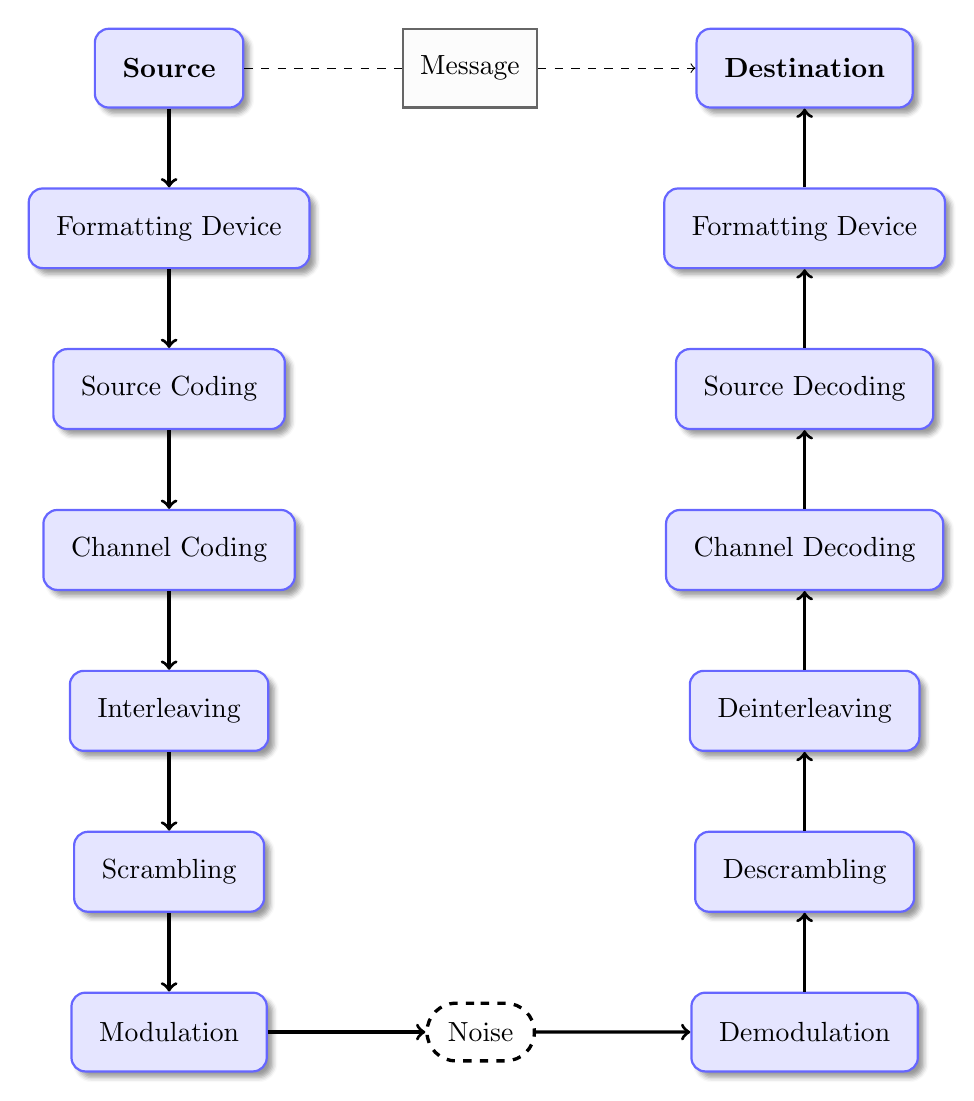
\begin{tikzpicture}[
        Step/.style = {rectangle, rounded corners = 5, inner sep = 10, draw = blue!60, fill = blue!10, thick, blur shadow, minimum size = 1cm},
        % 
        Noise/.style = {rounded rectangle, inner sep = 7, draw = black, dashed, very thick},
        % 
        Message/.style = {rectangle, draw = black!60, fill = black!1, thick, minimum width = 1.7cm, minimum height = 1cm },
    ]
        % Source
        \node[Step] (Source) {\textbf{Source}};
        \node[Step] (FormDevSou) [below = of Source] {Formatting Device};
        \node[Step] (SourceCoding) [below = of FormDevSou] {Source Coding};
        \node[Step] (ChanCod) [below = of SourceCoding] {Channel Coding};
        \node[Step] (Interleaving) [below = of ChanCod] {Interleaving};
        \node[Step] (Scrambling) [below = of Interleaving] {Scrambling};
        \node[Step] (Modulation) [below = of Scrambling] {Modulation};

        % Noise
        \node[Noise] (Noise) [right = 2cm of Modulation] {Noise};

        % Message
        \node[Message] (Message) [right = 2cm of Source] {Message};

        % Destination
        \node[Step] (Destination) [right = 2cm of Message] {\textbf{Destination}};
        \node[Step] (FormDevDest) [below = of Destination] {Formatting Device};
        \node[Step] (SourceDec) [below = of FormDevDest] {Source Decoding};
        \node[Step] (ChanDec) [below = of SourceDec] {Channel Decoding};
        \node[Step] (Deinterleaving) [below = of ChanDec] {Deinterleaving};
        \node[Step] (Descrambling) [below = of Deinterleaving] {Descrambling};
        \node[Step] (Demodulation) [below = of Descrambling] {Demodulation};
        



        % Arrow Message
        \draw[-, dashed] (Source) to node[]{} (Message);
        \draw[->, dashed] (Message) to node[]{} (Destination);


        % Arrows source
        \draw[->, very thick] (Source) to node[]{} (FormDevSou);
        \draw[->, very thick] (FormDevSou) to node[]{} (SourceCoding);
        \draw[->, very thick] (SourceCoding) to node[]{} (ChanCod);
        \draw[->, very thick] (ChanCod) to node[]{} (Interleaving);
        \draw[->, very thick] (Interleaving) to node[]{} (Scrambling);
        \draw[->, very thick] (Scrambling) to node[]{} (Modulation);

        % Noise
        \draw[->, very thick] (Modulation) to node[]{} (Noise);
        \draw[->, very thick] (Noise) to node[]{} (Demodulation);

        % Arrows destination
        \draw[->, very thick] (Demodulation) to node[]{} (Descrambling);
        \draw[->, very thick] (Descrambling) to node[]{} (Deinterleaving);
        \draw[->, very thick] (Deinterleaving) to node[]{} (ChanDec);
        \draw[->, very thick] (ChanDec) to node[]{} (SourceDec);
        \draw[->, very thick] (SourceDec) to node[]{} (FormDevDest);
        \draw[->, very thick] (FormDevDest) to node[]{} (Destination);

    \end{tikzpicture}
    \caption{The diagram of the digital information transmission system.}
    \label{fig:transmission_diagram}
\end{figure}
    % 
    % 
    \item \textsl{Noise.} The noise is a crucial obstacle to overcome to have a successful transmission; the noise is the main reason for a wrongly transmitted symbol. There are different types of noise, some of them are generated by other transmissions, others are due to the physical medium and others are caused by the intermediate devices between the transmission. Nevertheless, in every transmission, there will be the \textsl{Gaussiam White Noise} which is a thermal noise caused by the Big Bang.
    % 
    \item \textsl{Demodulation.} In this phase the demodulator device, after receiving the disturbed signal, will try to detect the signal to regenerate the original one. Sometimes the noise energy will be stronger than the signal energy generating errors that will be corrected in the next steps.
    % 
    \item \textsl{Descrambling.} The descrambling procedure is the opposite of the scrambling. The added \textit{pseudo-random sequence}, after the reception is subtracted by the descrambler.
    % 
    \item \textsl{Deinterleaving.} The deinterleaver reorders the transmitted symbols in the opposite way that the interleaver did. In such a way the \textit{burst} errors that occurred during the transmission will become single errors that can be easily recovered.
    % 
    \item \textsl{Channel Decoding.} 
    % 
    \item \textsl{Source Decoding.} The source decoding procedure decompresses the received data into the original symbols. This is achieved by one of the source coding properties: symbols are easily detected because there are no shorter codes at the beginning of longer codes.
    % 
    \item \textsl{Formatting Device.} During the transmission this device converts the signal from analogic to digital, during the reception of the signal the formatting device translates the discrete digital signal into a continuous analogic signal. 
    % 
    \item \textsl{Destination.} The destination device is whichever device will receive the signal. Likewise the source one, the destination device could be a satellite, a smartphone, a server, or anything else.
\end{itemize}

\subsection{Initial parameters}
The parameters used in this project have been assigned in a datasheet and are reported in the following list:
\vspace{-5px}
\begin{itemize}
    \renewcommand{\labelitemi}{$\cdot$}
    \setlength{\itemsep}{-2px}
    \item \textsl{Symbol duration}: 60 ns, also called $\tau$;
    \item \textsl{SNR}: 8.1 dB;
    \item \textsl{Source code}: Shannon-Fano coding;
    \item \textsl{Error correction code}: cyclic coding with codeword length \textit{m = 31} and generator polynomial $ z^5 \oplus z^2 \oplus 1$;
    \item \textsl{Carrier frequency}: 2.5 GHz;
    \item \textsl{Modulation}: Binary Amplitude Shift Keying (BPSK) with the phase shift of $\pi$.
\end{itemize}

\noindent In addition, the source data (alphabet) and the symbols' respective probabilities are summarized in the following table.

\begin{table}[h!]
    \centering
    \begin{tabular}{|c|c|}
        \hline
        \multicolumn{2}{|c|}{\texttt{Source 7}} \\\hline\hline
        $ a_1 $ & 0.11 \\
        $ a_2 $ & 0.07 \\
        $ a_3 $ & 0.09 \\
        $ a_4 $ & 0.01 \\
        $ a_5 $ & 0.06 \\
        $ a_6 $ & 0.06 \\
        $ a_7 $ & 0.13 \\
        $ a_8 $ & 0.14 \\
        $ a_9 $ & 0.13 \\
        $ a_{10} $ & 0.05 \\
        $ a_{11} $ & 0.11 \\
        $ a_{12} $ & 0.04 \\\hline
    \end{tabular}
    \label{tab:source7}
\end{table}

\noindent Afterwards the parameters have been transcripted in the MATLAB program, as shown in the following snippet. 

\begin{lstlisting}
% source number 7
ALPHABET = [1, 2, 3, 4, 5, 6, 7, 8, 9, 10, 11, 12];
PROBABILITY_VECTOR = [11, 7, 9, 1, 6, 6, 13, 14, 13, 5, 11, 4]/100;

TAU = 60e-9; % symbol duration time, [s]
SNR = 8.1; % Signal-to-Noise-Ration, [dB]
% Source Code: Shannon-Fano
% Error correction code: Cyclic
CODEWORD_LENGTH = 31; % m
% 
F_0 = 2.5e+9; % carrier frequency [Hz]
% Modulation: BPSK
PHASE_SHIFT = pi; % [rad]
U = 1; % amplitude BPSK signal [V]

transmitted_symbol_number = 20;
\end{lstlisting}





\setcounter{secnumdepth}{1}




\newpage \part{Analysis}

\section{Source data}

The source data analysis provides a general overview of how the data are generated and how this will impact the encoding scheme. Specifically, the source data analysis is achieved by calculating two important values: the source entropy and the redundancy coefficient.

\subsection{Source entropy}

The source entropy $H$ and the maximum source entropy $H_{\max}$. The entropy of a sequence of symbols is a number that summarizes the randomness of the selection of the symbols in the source sequence. The more uncertain the symbols are, the higher the entropy is and the higher the information the symbols carry. The ideal entropy is when the source symbols are \texttt{1 0 1 0 1 0 \dots} while the worst entropy is when all the symbols are \texttt{1} or \texttt{0}. Given a sequence $S$ of $N$ symbols, where each of them has its probability $P_i$ to occur, the entropy of the sequence is:

\begin{equation*}
    H(S) = - \sum_{i = 1}^{N}\,P_i \log_2 P_i
\end{equation*}

\noindent The entropy calculation can be simply achieved with the following MATLAB code. The only thing to note is that P is the probability vector that assigns to every symbol of the alphabet its probability. 

\begin{lstlisting}  
    % sum(V .* log2(V))
    H = - dot(PROBABILITY_VECTOR, log2(PROBABILITY_VECTOR));
\end{lstlisting}

\noindent Secondly, in order to calculate the maximum entropy $H_{\max}$, two conditions have to be met: all of the symbols have the same probability $P_i = \frac{1}{N}$ and, of course, they do not correlate one another. Consequently:

\begin{equation*}
    H_{\max}(S) = - \sum_{i = 1}^{N}\,\frac{1}{N} \log_2 \frac{1}{N} = \frac{1}{N} \sum_{i = 1}^{N}\, \log_2 N = \log_2N
\end{equation*}

\noindent Also in this case the MATLAB script to calculate the maximum entropy is trivial.

\begin{lstlisting}
    % Number of symbols in the alphabet
    N  = length(PROBABILITY_VECTOR);

    % Maximum source entropy
    H_max = log2(N);
\end{lstlisting}

\noindent By running the scripts, the value obtained are $H = 3.3995$ while $H_{\max} = 3.5850$. Reasonably $H < H_{\max}$ because the given probabilities in the datasheet weren't equal to each other.

% 
\subsection{Redundancy coefficient}

The redundancy coefficient $\rho$ summarizes in a number how much additional information is present inside the sequence. Essentially, the lower the redundancy coefficient is, the better, because it means that the source entropy is very high. Mathematically, the coefficient $\rho$ can be obtained as follows:

\begin{equation*}
    \rho = 1 - \frac{H}{H_{\max}}(S)    
\end{equation*}

\noindent which translates into the following code snippet:

\begin{lstlisting}
    % Calculate the redundancy coefficient 'rho'
    source_redoundancy = 1 - H/H_max;
\end{lstlisting}

\noindent Expectedly, the redundancy coefficient is not zero because $H<H_{\max}$: by running the script, $\rho = 0.0517$.



 % Task 2

\vspace{40px} \section{Source encoding} \label{source-encoding}
The source coding analysis provides the necessary tools to evaluate the source coding algorithms for efficient data representation and compression. In this case, the analysis calculates and uses different values to provide a better understanding of the efficiency of the Shannon-Fano source coding. Particularly the values that will be analyzed are the average codeword length $\overline{m}$, the probability of \texttt{1} and \texttt{0} ($P_1$ and $P_0$), the binary entropy $H_{bin}$, the source data generation rate $R$ and the compression ratio $K$.


\subsection{Shannon-Fano algorithm}
Before calculating the values it is important to encode the symbols of the alphabet through the Shannon-Fano algorithm. A brief recursive description of it is reported below.
\begin{enumerate}
    \item Sort the symbol of the alphabet by descending probability;
    \item Divide the sets of symbols into two continuous subsets with the same probability (or the lowest difference between the two);
    \item Assign to one subset the symbol 1 and the other 0;
    \item Repeat until every subset consists of one symbol;
    \item Read the codeword from left to right.
\end{enumerate} 

\noindent By applying the Shannon-Fano algorithm to the given source, the result should be the following.

\begin{table}[h]
    \centering
    \begin{tabular}{|c|c|c c c c c|c|c|c|c|}
        \hline
        \texttt{S} & \texttt{P} & \multicolumn{5}{c|}{Shannon-Fano} & \texttt{Code} & $m$ & $m_0$ & $m_1$ \\ \hline\hline
        $a_8$    & 0.14 & \cellcolor{teal!25} & \cellcolor{cyan!15} & 1 &  &  & \texttt{111} & 3 & 0 & 3\\
        $a_7$    & 0.13 & \cellcolor{teal!25} & \multirow[vpos]{-2}{*}{\cellcolor{cyan!15}1} & 0 &  &  & \texttt{110} & 3 & 1 & 2\\
        $a_9$    & 0.13 & \cellcolor{teal!25} & \cellcolor{cyan!20} & 1 &  &  & \texttt{101} & 3 & 1 & 2\\
        $a_1$    & 0.11 & \multirow[vpos]{-4}{*}{\cellcolor{teal!25}1} & \multirow[vpos]{-2}{*}{\cellcolor{cyan!20}1} & 0 &  &  & \texttt{100} & 3 & 2 & 1\\
        $a_{11}$ & 0.11 & \cellcolor{green!25} & \cellcolor{lime!25} & 1 &  &  & \texttt{011} & 3 & 1 & 2\\
        $a_3$    & 0.09 & \cellcolor{green!25} & \cellcolor{lime!25} & \cellcolor{lime!15} & 1 &  & \texttt{0101} & 4 & 2 & 2\\
        $a_2$    & 0.07 & \cellcolor{green!25} & \multirow[vpos]{-3}{*}{\cellcolor{lime!25}1} & \multirow[vpos]{-2}{*}{\cellcolor{lime!15}0} & 0 &  & \texttt{0100} & 4 & 3 & 1\\
        $a_5$    & 0.06 & \cellcolor{green!25} & \cellcolor{lime!35} & \cellcolor{yellow!25} & 1 &  & \texttt{0011} & 4 & 2 & 2\\
        $a_6$    & 0.06 & \cellcolor{green!25} & \cellcolor{lime!35} & \multirow[vpos]{-2}{*}{\cellcolor{yellow!25}1} & 0 &  & \texttt{0010} & 4 & 3 & 1\\
        $a_{10}$ & 0.05 & \cellcolor{green!25} & \cellcolor{lime!35} & \cellcolor{yellow!35} & 1 &  & \texttt{0001} & 4 & 3 & 1\\
        $a_{12}$ & 0.04 & \cellcolor{green!25} & \cellcolor{lime!35} & \cellcolor{yellow!35} & \cellcolor{orange!15} & 1 & \texttt{00001} & 5 & 4 & 1\\
        $a_4$    & 0.01 & \multirow[vpos]{-8}{*}{\cellcolor{green!25}0} & \multirow[vpos]{-5}{*}{\cellcolor{lime!35}0} & \multirow[vpos]{-3}{*}{\cellcolor{yellow!35}0} & \multirow[vpos]{-2}{*}{\cellcolor{orange!15}0} & 0 & \texttt{00000} & 5 & 5 & 0\\
        \hline
    \end{tabular}
    \label{tab:shannon-fano}
\end{table}

\FloatBarrier \noindent After computing the Shannon-Fano algorithm to the given source, the results should be inserted into the MATLAB program, as follows.

\begin{lstlisting}
% Probability vector sorted from highest to lowest
P = sort(PROBABILITY_VECTOR, 'descend');


% Values obtained with Shannon-Fano code algorithm

% Symbols codeword length
m = [3, 3, 3, 3, 3, 4, 4, 4, 4, 4, 5, 5]; 

% Number of 0s inside the symbols codeword
m_0 = [0, 1, 1, 2, 1, 2, 3, 2, 3, 3, 4, 5];

% Number of 1s inside the symbols codeword
m_1 = [3, 2, 2, 1, 2, 2, 1, 2, 1, 1, 1, 0];
\end{lstlisting}


\subsection{Binary entropy}
At this point, there is all the needed information to calculate the required data for the analysis. First of all, to calculate the average codeword length $\overline{m}$ of $N$ symbols, the following formula should be computed:

\begin{equation*}
    \overline{m} = \sum_{i = 1}^N\,m_i \cdot P_i 
\end{equation*}

\noindent Additionally, to calculate $P_0$ and $P_1$, it is necessary to calculate also the average number of 0 and 1 symbols. The formula is the same as for the average codeword length:

\begin{equation*}
    \overline{m_0} = \sum_{i = 1}^N\,m_{0_i} \cdot P_i 
    \hspace*{40px}
    \overline{m_1} = \sum_{i = 1}^N\,m_{1_i} \cdot P_i
\end{equation*}

\noindent After inserting these formulas in the MATLAB script, the values are $\overline{m} = 3.4300$, $\overline{m_0} = 1.6400$ and $\overline{m_1} = 1.7900$.

\begin{lstlisting}
% Average codeword length
m_average = dot(P, m); 

% Average number of 0 symbols
m_0_average = dot(P, m_0);

% Average number of 1 symbols
m_1_average = dot(P, m_1);
\end{lstlisting}


\noindent Moreover, by dividing the number of 0 or 1 symbols by the average length of the codeword the two probabilities, $P_0$ and $P_1$, can be computed:

\begin{equation*}
    P_0 = \frac{\overline{m_0}}{\overline{m}}
    \hspace*{40px}
    P_1 = \frac{\overline{m_1}}{\overline{m}}
\end{equation*}

\noindent The two probabilities values are $P_0 = 0.4781$ and $P_1 = 0.5219$. Ideally, the probabilities should be $P_0 = P_1 = 0.5$; nonetheless, the two values are still very close to each other. Finally, with the two probability values the binary entropy $H_{bin}$ can be obtained using the following calculation.

\begin{equation*}
    H_{bin}(S) = - P_0\log_2P_0 - P_1\log_2P_1
\end{equation*}

\noindent By running the following MATLAB script, the value of the binary entropy is $H_{bin} = 0.9986$ which is very close to 1. The higher the entropy is, the more uncertainty is associated with every symbol: this means that encoding the initial data with the Shannon-Fano algorithm provides a great value, information-wise.

\begin{lstlisting}
% Probability of 0 symbol
P_0 = m_0_average / m_average; 

% Probability of 1 symbol
P_1 = m_1_average / m_average; 

% Binary source entropy after coding
H_bin = -P_0 * log2(P_0) - P_1 * log2(P_1); 
\end{lstlisting}


\subsection{Data rate and compression ratio}
After encoding the source data with the Shannon-Fano algorithm, it is important to evaluate the source data generation rate $R$, which can be calculated as follows:

\begin{equation*}
    R = \frac{H(S)}{\overline{m}\tau}\text{, where $\tau$ is the symbol duration}
\end{equation*}
 
\noindent The data compression ratio $K$ is important as well: it helps evaluate how much the initial data has been compressed after the source coding. The following formula will help to obtain this value.

\begin{equation*}
    K = \frac{\overline{m}}{H(S)}
\end{equation*}

\noindent After running the MATLAB script displayed below, the data rate $R = 16.519 Mbit/s$ which should be lower than the channel capacity $C_{chan}$ with noise. Moreover, the compression ratio $K = 1.0090$ which is very close to 1, means that the overall compression is low: this is still not a bad result because the overall entropy is increased significantly after the source coding.

\begin{lstlisting}
% Calculate Data Rate
R = H * (m_average * TAU) ^ (-1);

% Calculate Compression Ratio
K = m_average / H;
\end{lstlisting}
 % Task 3

\vspace{40px} \section{Shannon's theorem condition}

 % Task 4

% 

\setcounter{secnumdepth}{0}
\vspace{40px}\section{Raw results}\label{raw-results}
\todo{Make a little introduction in the "Raw result" section}

\begin{center}
\renewcommand{\arraystretch}{1.5}
\begin{longtable}{|c|c|c|}
    
    \hline \multicolumn{1}{|c|}{\textbf{Symbol}} & \multicolumn{1}{c|}{\textbf{Description}} & \multicolumn{1}{c|}{\textbf{Value}} \\ \hline 
    \endfirsthead

    \multicolumn{3}{r}%
    {{\small\textit{\dots continued from previous page}}} \\
    \hline \multicolumn{1}{|c|}{\textbf{Symbol}} & \multicolumn{1}{c|}{\textbf{Description}} & \multicolumn{1}{c|}{\textbf{Value}} \\ \hline 
    \endhead

    \hline \multicolumn{3}{l}{{\small\textit{Conitnue on next page \dots}}}
    \endfoot

    \hline\endlastfoot

    
    \multicolumn{3}{|c|}{\textit{Task 2}} \\\hline
    $H(S)$ & Source entropy & 3.3995 \\
    $H(S)_{max}$ & Maximum source entropy & 3.5850 \\
    $\rho$ & Source redundancy & 0.0517 \\

    \hline\multicolumn{3}{|c|}{\textit{Task 3}} \\\hline
    $\overline{m}$ & Average codeword length & 3.4300 \\
    $P_0$ & Probability of \texttt{"0"} & 0.4781 \\
    $P_1$ & Probability of \texttt{"1"} & 0.5219 \\
    $H_{bin}(S)$ & Binary entropy & 0.9986 \\
    $R$ & Source data rate & 16.519 Mbps \\
    $K$ & Compression ratio & 1.0090 \\

    \hline\multicolumn{3}{|c|}{\textit{Task 4}} \\\hline
    $C_{bin}$ & Noiseless channel capacity & 16.667 Mbps \\
    $P_{err}$ & Error probability (BER) & $1.6315 \cdot 10^{-4}$ \\
    $C_{chan}$ & Channel capacity with noise & 16.629 Mbps \\

    \hline\multicolumn{3}{|c|}{\textit{Task 5}} \\\hline


    \hline\multicolumn{3}{|c|}{\textit{Task 6}} \\\hline


    \hline\multicolumn{3}{|c|}{\textit{Task 7}} \\\hline


    \hline\multicolumn{3}{|c|}{\textit{Task 8}} \\
    $P_{>2\,err}$ & Probability of $>2$ errors occurring & $ 1.2338\cdot10^{-5} $ \\

    \end{longtable}
\renewcommand{\arraystretch}{1}
\end{center}







\setcounter{secnumdepth}{1} % Summary


% ==================================================
\setcounter{section}{0}

\newpage \part{Simulation}

\section{Data generation algorithm}
To simulate the transmission using the given \hyperref[initial-parameters]{initial parameters} it is crucial to generate the symbols following the probabilities specified in the \hyperref[tab:source7]{\texttt{Source 7}} data sheet. To achieve such generation specifics a generation algorithm shall be implemented in MATLAB. The following MATLAB functions will generate a sequence of \texttt{n} symbols in the alphabet following their probability distribution.  

\subsection{Comulative distribution probabilities calculator}
The first function - \texttt{distribution\_probability\_matrix} - will take as input the \texttt{symbol\_matrix} whose first row contains the symbols in the alphabet and the second row contains their respective probabilities. The function will return a matrix whose first row is the same but the second row contains cumulative distribution meaning that the second probability value is added to the first, the third is added to the second and so on. Consequently, the last probability value will be one.

\begin{lstlisting}
function result = distribution_probability_matrix(symbol_matrix)
    % Extract probability vector from the symbol matrix
    probability_vector = symbol_matrix(2, :);
    
    % Get the number of possible symbols
    alphabet_length = length(probability_vector);

    % Calculate the cumulative probability matrix
    cumulative_probability = 0;
    sum_probability_vector = zeros(1, alphabet_length);
    for i = 1:alphabet_length
        % Calculate cumulative probability
        cumulative_probability = cumulative_probability + probability_vector(i);
        
        % Store cumulative probability in the vector
        sum_probability_vector(i) = cumulative_probability;
    end

    % Combine symbols and cumulative probabilities into the result matrix
    result = [symbol_matrix(1, :); sum_probability_vector];
end
\end{lstlisting}

\noindent This helper function will be useful when a random number $r$ between 0 and 1 is generated: the symbol associated with $r$ will be the $i$-th symbol where $P_{i-1} < r \leq P_i$. In such a way the symbols will have the same probability to be associated with the number $r$ as specified in the \hyperref[tab:source7]{datasheet}.


\subsection{Sequence generator}
The \texttt{distribution\_probability\_matrix} function will be used in the actual generation function called \texttt{symbol\_sequence\_generator} which generates \texttt{n} symbols conforming with their specified probabilities. The below-displayed function will generate a random number $r$ between 0 and 1 and associate it with the $i$-th symbol whose probability is $P_{i-1} < r \leq P_i$. This is achieved by subtracting the random number from the cumulative probability vector and choosing the symbol with the lowest positive probability value. This procedure is computed \texttt{n} time: every temporal association is added to the final result which will be the generated symbol sequence.

\begin{lstlisting}
function result = symbol_sequence_generator(symbol_matrix, n)
    % Initialize an empty vector for the symbol sequence with length n
    result = zeros(1, n);

    % Calculate the cumulative probability matrix using the provided function
    sum_probability_matrix = distribution_probability_matrix(symbol_matrix);
    
    % Generate the symbol sequence
    for i = 1:n
        % Generate a random number between 0.00 and 1.00
        random_number = round(rand(), 2);
        
        % Calculate the distance of each cumulative probability from the random number
        distance_from_random_number = sum_probability_matrix(2, :) - random_number;
        distance_from_random_number(distance_from_random_number < 0) = +Inf;

        % Get the index of the symbol with the minimum distance
        [~, symbol] = min(distance_from_random_number);
        
        % Assign the selected symbol to the result vector
        result(i) = symbol;
    end
end
\end{lstlisting}

\vspace{40px} \section{Source coding and decoding}
The second step is to implement an algorithm that will encode and decode the newly generated symbols using the Shannon-Fano algorithm. The two algorithms are based on the results obtained and displayed in the \texttt{Code} column of the \hyperref[tab:shannon-fano]{table} in the \hyperref[source-encoding]{"Source encoding" section}.

\subsection{Shannon-Fano encoding}\label{source-coding}
The Shannon-Fano encoding can be achieved by using a very simple switch. Sure enough, the helper function \texttt{encode\_symbol} displayed below associates with every symbol in the alphabet and its respective codeword.

\begin{lstlisting}
function result = encode_symbol(symbol)
    % Use a switch statement to assign the encoded representation based on the input symbol
    switch symbol
        case 1
            result = [ 1 0 0 ];
        case 2
            result = [ 0 1 0 0 ];
        case 3 
            result = [ 0 1 0 1 ];
        case 4 
            result = [ 0 0 0 0 0 ];
        case 5 
            result = [ 0 0 1 1 ];
        case 6 
            result = [ 0 0 1 0 ];
        case 7 
            result = [ 1 1 0 ];
        case 8 
            result = [ 1 1 1 ];
        case 9 
            result = [ 1 0 1 ];
        case 10 
            result = [ 0 0 0 1 ];
        case 11 
            result = [ 0 1 1 ];
        case 12
            result = [ 0 0 0 0 1 ];
    end
end
\end{lstlisting}

\noindent The \texttt{shannon\_fano\_encoding} function takes the \texttt{symbol\_sequence} as input and encodes it symbol-by-symbol using the aforementioned \texttt{encode\_symbol} function.

\begin{lstlisting}
function encoded_sequence = shannon_fano_encoding(symbol_sequence)
    encoded_sequence = [];
    
    % Iterate through the symbol sequence and encode each symbol
    for i = 1:length(symbol_sequence)
        encoded_sequence = [encoded_sequence, encode_symbol(symbol_sequence(i))];
    end
end
\end{lstlisting}

\subsection{Shannon-Fano decoding}\label{source-decoding}
The decoding algorithm performs the exact reverse operation of the encoding algorithm. Sure enough, there is the \texttt{decode\_symbol} function which translates the binary sequence into its respective symbol.
\begin{lstlisting}
function symbol = decode_symbol(code)
    % Use a switch statement to check each possible code and return the corresponding symbol
    switch code
        case '[1 0 0]'
            symbol = 1;
        case '[0 1 0 0]'
            symbol = 2;
        case '[0 1 0 1]'
            symbol = 3;
        case '[0 0 0 0 0]'
            symbol = 4;
        case '[0 0 1 1]'
            symbol = 5;
        case '[0 0 1 0]'
            symbol = 6;
        case '[1 1 0]'
            symbol = 7;
        case '[1 1 1]'
            symbol = 8;
        case '[1 0 1]'
            symbol = 9;
        case '[0 0 0 1]'
            symbol = 10;
        case '[0 1 1]'
            symbol = 11;
        case '[0 0 0 0 1]'
            symbol = 12;
        otherwise
            symbol = []; % Return empty if the code does not match any known code
    end
end
\end{lstlisting}

\noindent This function is used in the \texttt{shannon\_fano\_decoding} function wich performs the decoding of the input \texttt{encoded\_sequence}. The body of the function is a little more complicated than the encoding function because the length of the encoded symbol is not fixed - it can be 3, 4 or 5 - and, as such, every time a new symbol is read from the decoded data, a check should be done to understand if the symbol can be decoded or not. 

\begin{lstlisting}
function decoded_sequence = shannon_fano_decoding(encoded_sequence)
    decoded_sequence = [];
    
    % Iterate through the encoded sequence and decode each symbol
    current_code = [];
    for i = 1:length(encoded_sequence)
        current_code = [current_code, encoded_sequence(i)];
        
        % Check if the current code matches any known code
        symbol = decode_symbol(string(mat2str(current_code)));
        
        % If a symbol is found, add it to the decoded sequence and reset the current code
        if ~isempty(symbol)
            decoded_sequence = [decoded_sequence, symbol];
            current_code = [];
        end
    end
end
\end{lstlisting}


\vspace{40px} \section{Channel coding and decoding}
The Hamming encoding and decoding is the most crucial part of the transmission because it is the one responsible for the error correction of the transmission. There are two types of hamming encoding, group coding and cyclic coding: in this case, cyclic coding has been utilized to perform the error correction. It is important to note that the channel coding adds some bits to the codeword: precisely during the encoding phase to the codeword are added 5 symbols, making the sequence length a perfect divisor of $26 + 5 = 31$, meanwhile after the decoding the five symbols at the end of the codeword are removed making it again a perfect divisor of 26.   




\subsection{Cyclic Hamming encoding}
To perform the Hamming encoding to the sequence it is necessary to generate the \texttt{encoding\_matrix} using the \texttt{cyclgen} function\footnote{Note that the function needs to be imported: \texttt{import communications.*}.} that uses the codeword length and the generation polynomial defined at the \hyperref[initial-parameters]{beginning of the code}. The \texttt{hamming\_encoding} function, uses the generated encoding matrix to perform a matrix multiplication and encode the codeword.

\begin{lstlisting}
function encoded_data_matrix = hamming_encoding(binary_data_matrix, codeword_length, k, generation_polynomial)
    % Calculate the number of redundant symbols (parity symbols)
    r = codeword_length - k;
    
    % Generate the cyclic encoding matrix based on the generator polynomial
    [~, cyclic_encoding_matrix] = cyclgen(codeword_length, generation_polynomial);
    
    % Reorder the encoding matrix to match Hamming code requirements
    reorder = [r + 1 : codeword_length, 1 : r];
    cyclic_encoding_matrix = cyclic_encoding_matrix(:, reorder);
    
    % Calculate control symbol values using matrix multiplication
    % Use rem() function to find modulo 2 sum as a remainder of division by 2
    encoded_data_matrix = rem(binary_data_matrix * cyclic_encoding_matrix, 2);
end
\end{lstlisting}


\subsection{Cyclic Hamming decoding}
\todo{Finish here maybe arrange the function with other helper functions to help readibility}


\begin{lstlisting}
    function decoded_data_matrix = hamming_decoding(encoded_data_matrix, codeword_length, k, generation_polynomial)
        % Determine the number of control symbols
        r = codeword_length - k;
        
        % Specify syndrome calculation matrix
        [~, cyclic_encoding_matrix] = cyclgen(codeword_length, generation_polynomial);
        syndrome_matrix = cyclic_encoding_matrix(:, (1:r));
        syndrome_matrix = [syndrome_matrix; eye(r)];
        
        % Calculate syndrome for each codeword
        syndrome_value = rem(encoded_data_matrix * syndrome_matrix, 2);
        syndrome_value = syndrome_value * 2.^(r - 1 : -1 : 0)';
        
    
        % Define associations between syndrome values and error positions
        positions = (1 : codeword_length)'; 
    
        % Initialize vector to store decimal values of binary syndrome patterns
        syndrome_decimal_value_vector = [];
    
        % Convert binary syndrome values to decimal for association
        for i = 1 : codeword_length
            syndrome_decimal_value_vector = [syndrome_decimal_value_vector; bin2dec(num2str(syndrome_matrix(i, :)))];
        end
    
        % Combine positions and corresponding decimal values for sorting
        associations = [positions, syndrome_decimal_value_vector];
    
        % Sort associations based on decimal values for efficient error detection
        associations = sortrows(associations, 2);
    
        % Create correction index for mapping syndrome values to error positions
        correction_index = [0, associations(:, 1)'];
    
        % Map syndrome values to error positions using correction index
        error_indexes = correction_index(syndrome_value + 1);
        
    
        % Define error vector table
        error_vector = [zeros(1, codeword_length);
                        eye(codeword_length)];
        
        % Perform correction by adding the error vector to the received codeword
        codeword = rem(encoded_data_matrix + error_vector(error_indexes + 1, :), 2);
        
        % Read the columns of data symbols to form decoded data
        decoded_data_matrix = codeword(:, 1:k);
    end
\end{lstlisting}

This code is able to correcto only one error per codeword. This is why the interleaving process is needed to prevent any types of group errors.


\vspace{40px} \section{Interleaving and deinterleaving}
The interleaving and deinterleaving process is needed to prevent group errors, also called \textsl{burst errors}. This is achieved by deterministically mixing the sequence before the transmission and recomposing it by performing the initial algorithm in reverse. In such a way, if during the communication a burst error happens when the sequence is restored in the initial order, the possibility of having these types of errors drastically decreases.


\subsection{Interleaving}


\begin{lstlisting}
function mixed_sequence = interleaving(unmixed_sequence)
    % Define the length of each column (also the number of rows)
    column_length = 31;

    % Calculate the number of length of each row (also the number of columns) based on the input sequence length
    row_length = length(unmixed_sequence) / column_length;

    % Write on the columns and read on the rows to create the interleaved matrix
    interleaver_matrix = [];

    % Iterate through the rows
    for i = 1 : row_length
        % Extract the current column from the unmixed sequence
        current_column = unmixed_sequence(column_length * (i-1) + 1 : column_length * i)';
        
        % Append the current column to the matrix
        interleaver_matrix = [interleaver_matrix, current_column];
    end
    
    % Initialize the interleaved sequence
    mixed_sequence = [];

    % Iterate through the columns of the matrix
    for i = 1 : column_length
        % Append the elements from each row of the current column to the interleaved sequence
        mixed_sequence = [mixed_sequence, interleaver_matrix(i, 1 : end)];
    end

end
\end{lstlisting}

\subsection{Deinterleaving}


\vspace{40px} \section{Scrambling and descrambling}
The scrambling process helps with the synchronization between the sender machine and the receiver device. More precisely, when there is a long sequence of \texttt{"0"} or \texttt{"1"} symbols it becomes rather difficult to understand how many of them are being transmitted. For this purpose, before modulating and transmitting the signal, is extremely helpful to perform a logical \texttt{XOR} to every codeword with a pseudo-random sequence, called \texttt{scambling\_key}. This is the purpose of the \texttt{scrambling} function: it applies an exclusive \texttt{OR} bitwise with a key that is known both from the source and the destination.

\begin{lstlisting}
function scrambled_sequence = scrambling(unscrambled_sequence, scrambler_key)
    % Initialize the output sequence
    scrambled_sequence = [];

    % Determine the length of the scrambler key
    codeword_length = length(scrambler_key);

    % Loop through the input sequence in codeword-sized chunks
    for i = 1 : length(unscrambled_sequence) / codeword_length
        % Extract the current codeword from the input sequence
        current_codeword = unscrambled_sequence(codeword_length * (i - 1) + 1 : codeword_length * i);
        
        % Perform XOR operation with the scrambler key
        scrambled_codeword = xor(current_codeword, scrambler_key);

        % Append the scrambled codeword to the output sequence
        scrambled_sequence = [scrambled_sequence, scrambled_codeword];
    end
end
\end{lstlisting}

\noindent There is no need to create the \texttt{descrambling} function because the \texttt{XOR} operation is cyclical: performing this operation two times to a sequence of binary numbers will return the initial sequence. In this case, the function has been created just for better clarity and readability.

\begin{lstlisting}
function unscrambled_sequence = descrambling(scrambled_sequence, scrambler_key)
    % Utilize the scrambling function in reverse to perform descrambling
    unscrambled_sequence = scrambling(scrambled_sequence, scrambler_key);
end
\end{lstlisting}



\vspace{40px} \section{Modulation and noise}\label{modulation}
After translating, coding, mixing and changing the sequence it is finally time to simulate the signal transmission process. In this case, the Binary Phase Shift Keying has been utilized to modulate and demodulate the binary sequence. To create this type of signal, it is necessary to create the \texttt{carrier\_signal} which is a sine wave with the properties given in the \hyperref[initial-parameters]{initial parameters}. Then the carrier signal energy and its length are stored to calculate the Gaussian White Noise afterwards. The BPSK modulation is performed by creating an \textsl{NRZ} signal of the sequence and then using the \textit{Kronecker} product as shown below.

\begin{lstlisting}
    % Define the time-step
    delta_t = tau / samples_per_symbol;
    
    % Time intervals for one symbol
    time_intervals = 0: delta_t: tau - delta_t;
    
    % Create the carrier signal
    carrier_signal = sin(2 * pi * f0 * time_intervals);
    
    % Calculate the energy per symbol
    Eb = dot(carrier_signal, carrier_signal);
    
    % Save length of encoded sequence
    N = length(binary_sequence);
    
    % Perform BPSK modulation
    BPSK_signal = kron(-2 * binary_sequence + 1, carrier_signal);

\end{lstlisting}

\label{noise}\noindent To add the GWN is necessary to calculate the noise signal by reversing the SNR formula to obtain the noise spectral power density $N_0$. With this value, it is possible to obtain the standard deviation, $\sigma$ and then generate the \texttt{noise\_signal} which will be added to the modulated signal to compute the \texttt{disturbed\_signal}.

\begin{lstlisting}
    % Reversed SNR formula
    EbN0 = 10^(SNR / 10);
    
    % Obtain noise spectral power density
    N0 = Eb./EbN0;
    
    % Calculate sigma for BPSK
    sigma = sqrt(N0 / 2);
    
    % Create noise signal
    noise_signal = sigma * randn(1, N * samples_per_symbol);
    
    % Create disturbed signal by adding noise to the modulated signal
    disturbed_signal = BPSK_signal + noise_signal;
\end{lstlisting}

\label{demodulation}\noindent The signal detection is performed using the \textsl{correlation receiver} approach. The disturbed signal is sliced and then it is compared to its respective modulation threshold, which is 0 in this case.

\begin{lstlisting}
    % Slice the received signal into segments in each column
    sliced_disturbed_signal = reshape(disturbed_signal, samples_per_symbol, N);
    
    % Detect the signal with the BPSK threshold
    detected_signal = carrier_signal * sliced_disturbed_signal < 0;
\end{lstlisting}





\end{document}
